\section{Fazit}

In dieser Arbeit haben wir versucht, mithilfe von Grafana, Loki und Promtail eine \gls{SIEM} Lösung zu emulieren, um Überwachungsmechanismen anhand von Logdateien zu erstellen. In der folgenden Tabelle zeigen wir die Rolle jedes vewendeten Tools, um unser Ziel zu erreichen

\begin{table}[h]
    \centering
    \setstretch{1.2}
    \begin{tabular}{|c|c|}
    \hline
    \textbf{Funktionalität}         & \textbf{Tool}    \\ \hline
    Datensammlung                   & Promtail         \\ \hline
    Normalisierung und Vearbeitung  & Loki             \\ \hline
    Berichts- und Grafikgenerierung & Grafana          \\ \hline
    Generierung von Warnmeldung     & Grafana:Alerting \\ \hline
    \end{tabular}
    \caption{Verwendete Tools für den Aufbau einer \gls{SIEM} ähnlichen Lösung\\Quelle: Eigene Quelle und \citep{Granadillo_SIEM}}
    \label{tab:my-table}
\end{table}

Wir stellen fest, dass die verwendeten Tools eine kosteneffektive Möglichkeit bieten, ein Überwachungssystem zu implementieren. Die Methoden zur Erkennung von Angriffen lassen sich anhand der \gls{ttp} der \gls{mitre}-Matrix definieren. Nach der Auswahl des Angriffe erstellen wir Regelwerke mit der Abfragesprache \gls{logql} in Loki, um Muster zu identifizieren, die auf den ausgewählten Angriff hindeuten. Diese Regelwerke werden dann verwendet, um Warnmeldungen über den Angriff zu generieren und zu versenden.

\subsection{Herausforderungen}

Unser Aufbau birgt zwei große Herausforderungen, wobei die erste einfacher zu bewältigen ist als die zweite. Diese sind:

\subsubsection{Definition der Regelsätzen}
Für eine präzise Implementierung spielt die richtige Entwicklung der Regelsätzen zur Identifizierung potenzieller Angriffe eine wesentliche Rolle. Da Logdateien aus produktiven Umgebungen eine große Menge an Informationen enthalten, müssen diese Regelsätzen so definiert werden, dass sie die eindeutigen Informationen wie IP-Adresse, Portnummer, Zeitfenster und Zeitabstände zwischen Anfragen filtern und nach Angriffsmustern kategorisieren können.

\begin{itemize}[noitemsep]
    \item \textbf{Erkennung von \gls{KI}-basierte Angriffe:}
\end{itemize}
\subsubsection{Erkennung von \gls{KI}-basierte Angriffe}

Die von uns definierten Regeln haben statische Elemente wie die \quotes{Anzahl von Anfragen}, den \quotes{Zeitabstand zwischen Requests} und die \quotes{Anzahl von fehlgeschlagenen Anmeldeversuchen}. Die heutigen Angriffe haben jedoch auch einen dynamischen Aspekt, der sich an die Umgebung anpasst, insbesondere durch die starke Entwicklung von \glsfirst{KI} \citep{Guembe_AIHACKER}. Während \gls{KI} einerseits für die Automatisierung von Aufgaben oder für effiziente Datenanalyse verwendet wird, könnte sie auch für Cyberkriminalität genutzt werden. \gls{KI} ist am Ende nur ein Werkzeug, dessen Nutzung von den Absichten ihrer Benutzer abhängt.

Verschiedene Angriffstechniken lassen sich schneller und effizienter mit \gls{KI} durchführen. Die Nutzung von \gls{polyphomicMalware} ist ein Beispiel, wo weder Antivirus-Programme noch Log-Analyse-Tools einen normalen von einem abnormalen Ablauf unterscheiden können. Auch die Verkehrsanalyse kann durch \gls{KI} gefährdet sein, da Angriffe und normaler Verkehr ähnlich dargestellt werden können. Darüber hinaus kann \gls{KI} auch gegen Authentifizierungsverfahren eingesetzt werden, um beispielsweise Anmeldedaten schneller zu \gls{bruteforce} und/oder vorauszusehen \citep{Fritsch_AIcybersec}.

% \newpage
% Das folgende Diagramm zeigt, wo sich \gls{KI} bei Cyberangriffen anhand der\gls{CKC} integrieren lässt:


% \begin{figure}[H]
%     \centering
%     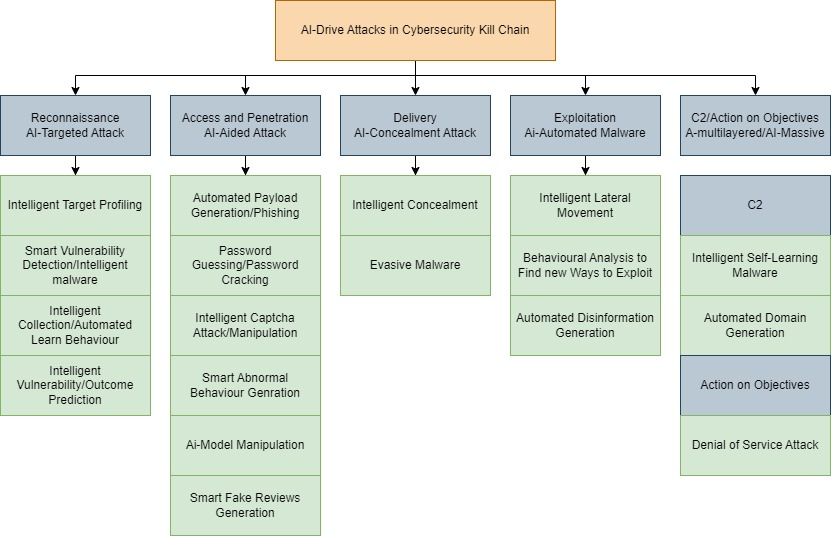
\includegraphics[width=0.9\textwidth]{assets//CKC_AI.jpg}
%     \caption[\gls{KI} in der \glsfirst{CKC}]
%     {\gls{KI} in der \glsfirst{CKC}\\Quelle: \citep{Guembe_AIDiagrammAngriff}}
%     \centering
%  \end{figure}
 
% \subsection{Zukünftige Recherche}
% Um sicherzustellen, dass unsere Lösungen sich an diese neue und dynamische Realität anpassen können, können zukünftige Regelsätze mithilfe von \gls{KI} erstellt werden. Nachdem die meisten möglichen Angriffsflächen identifiziert wurden, sollten die Regeln die viele mögliche Szenarien abdecken.

% Mit der rasanten Entwicklung von \gls{KI}, insbesondere während der Erstellung dieser Arbeit, können wir auch erwarten, dass sich sowohl Loki als auch Grafana bald mit verschiedenen \gls{opensource} \gls{plugin} integrieren lassen, die auch \gls{KI} unterstützen. Diese sollen dazu beitragen, die Loganalyse effizienter und zuverlässiger zu machen. All dies würde dabei helfen, einen sicheren Netzwerkverkehr zu gewährleisten.


